\documentclass[../tesis_main.tex]{subfiles}

\newpage{}

\vspace{0.7in}

\chapter*{Resumen}
\pagenumbering{roman}
\section*{}

\pagenumbering{roman}
\setcounter{page}{7}
	El reconocimiento de objetos y la adecuada manipulación de los mismos es una problemática común en el área de la robótica de servicios. El presente documento aborda el diseño de un sistema de manipulación de objetos formado por un manipulador de 7DOF, el desarrollo de un algoritmo de visión computacional para obtener la posición y orientación de los objetos, la puesta a prueba de diferentes algoritmos para el cálculo de la cinemática inversa del brazo robótico y finalmente la planeación de acciones entre la detección de un objeto y su correcta manipulación.\\

	El desarrollo del sistema de manipulación se plantea con diferentes subtareas, se comienza con la descripción de la detección de objetos utilizando el algoritmo RANSAC para encontrar superficies planas, se plantea un algoritmo para la extracción de objetos, posteriormente se plantea un análisis de componentes principales para estimar la orientación de los objetos sobre el plano.\\

	Se continua con la descripción del manipulador de 7DOF, se analiza la cinemática directa haciendo énfasis en la caracterización experimental del espacio de trabajo del manipulador y se reportan algoritmos utilizados para el cálculo de la cinemática inversa.\\

	Posteriormente se reporta la integración del sistema utilizando la plataforma ROS (Robot Operative System), finalmente concluye con la descripción de la tarea de manipulación de objetos y se reportan resultados y conclusiones.\\

	Los algoritmos desarrollados en el presente documento pueden ser utilizados en la segmentación de objetos de manera general, y podrán ser implementados para realizar un seguimiento de peatones o usuarios de bicicletas en un sistema de monitoreo para bicicletas ecológicas como parte del proyecto "Laboratorio de Movilidad e Infraestructura Verde para la Eficiencia Energética en Ciudades".\\

\newpage
\thispagestyle{empty}

\chapter{Introducción}
\pagenumbering{arabic}
	%¿Por qué son importantes los robots de servicio?
	En los últimos años, el área de la robótica y sus múltiples aplicaciones se han expandido a pasos agigantados, tal es el caso de la robótica de servicios. Años atrás la idea de tener un robot capaz de ayudar en las tareas del hogar sólo era concebida gracias a la ciencia ficción; hoy en día es una total realidad. 
	%Robot definition
	Un robot inteligente es una máquina capaz de extraer información de su entorno y usar su conocimiento del mundo para moverse con seguridad de manera significativa y deliberada.\cite{arkin1998behavior} Actualmente existe un auge en utilizar a los robots como auxiliares en las actividades domesticas, un área llamada: ``robótica de servicio''. Sin embargo, el área de la robótica de servicios y robots de asistencia comprende un gran rango de problemáticas.\\

	Es conveniente poner en contexto algunas definiciones útiles según la Federación Internacional de Robótica. Un \textbf{robot de servicio} es un robot que realiza tareas útiles para humanos o equipos, excluida la aplicación de automatización industrial \cite{IFREpage}. Un \textbf{robot de servicio personal} o un \textbf{robot de servicio para uso personal} es un robot de servicio utilizado para una tarea no comercial, por lo general por personas con alguna limitación física. Algunos ejemplos son el robot de servicio doméstico, la silla de ruedas automatizada y el robot de asistencia de movilidad personal\cite{IFREpage}.\\

	La motivación de este trabajo se encuentra en las condiciones de la población con alguna discapacidad en México. De acuerdo con el INEGI y SEDESOL, en México, hasta el 2014, el 6.4$\%$ de la población reportó alguna discapacidad. La mayoría son personas adultas mayores y los principales tipos de discapacidad son la motriz, la visual y los problemas para aprender, recordar o concentrarse\cite{sedesolEpage}. Respecto al uso de ayudas técnicas para personas con discapacidad, sólo se menciona el uso de lentes para los problemas de visión. Para los problemas de movilidad las personas con discapacidad reportan usar bastón, silla de ruedas, muletas, andaderas, la ayuda de alguien y otros \cite{inegiEpage}.\\

	\begin{figure}[H]
		\begin{subfigure}[t]{.5\textwidth}
		\centering{}
		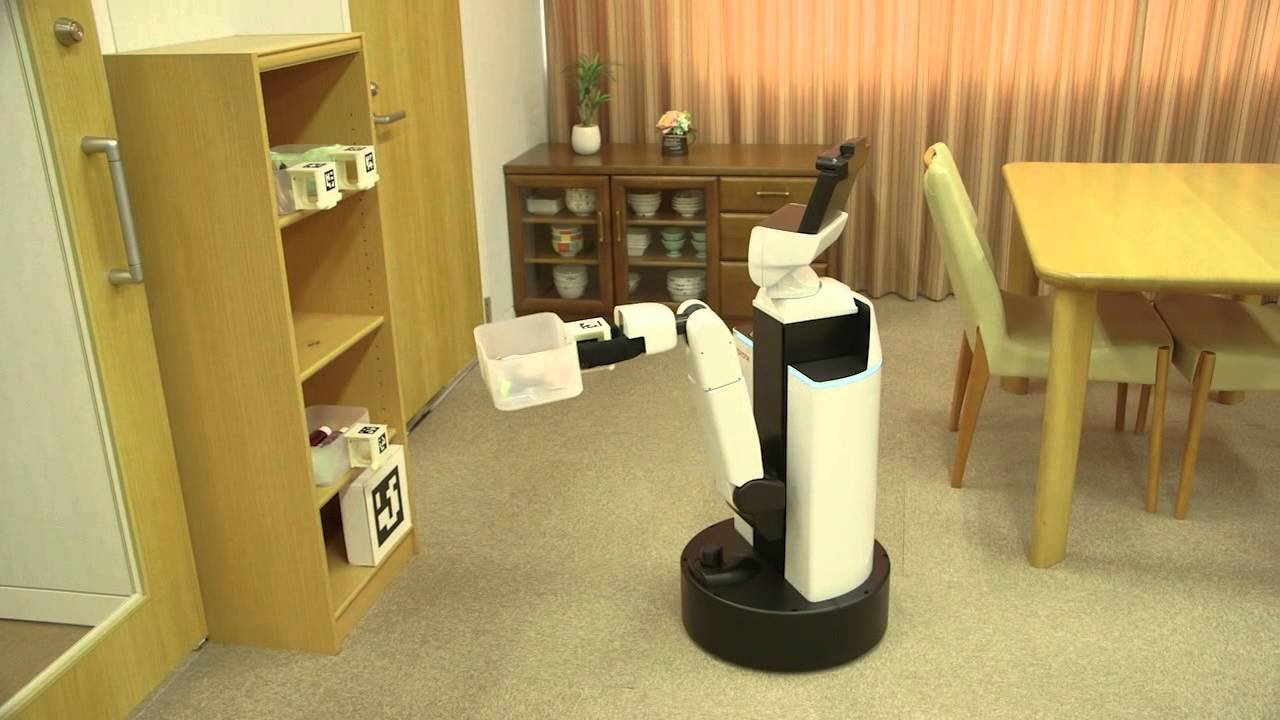
\includegraphics[width=5.0cm, height=3.5cm]{estadoArte/hsr_human_assistant.jpg}	
		\end{subfigure}%
		\begin{subfigure}[t]{.5\textwidth}
		\centering{}
		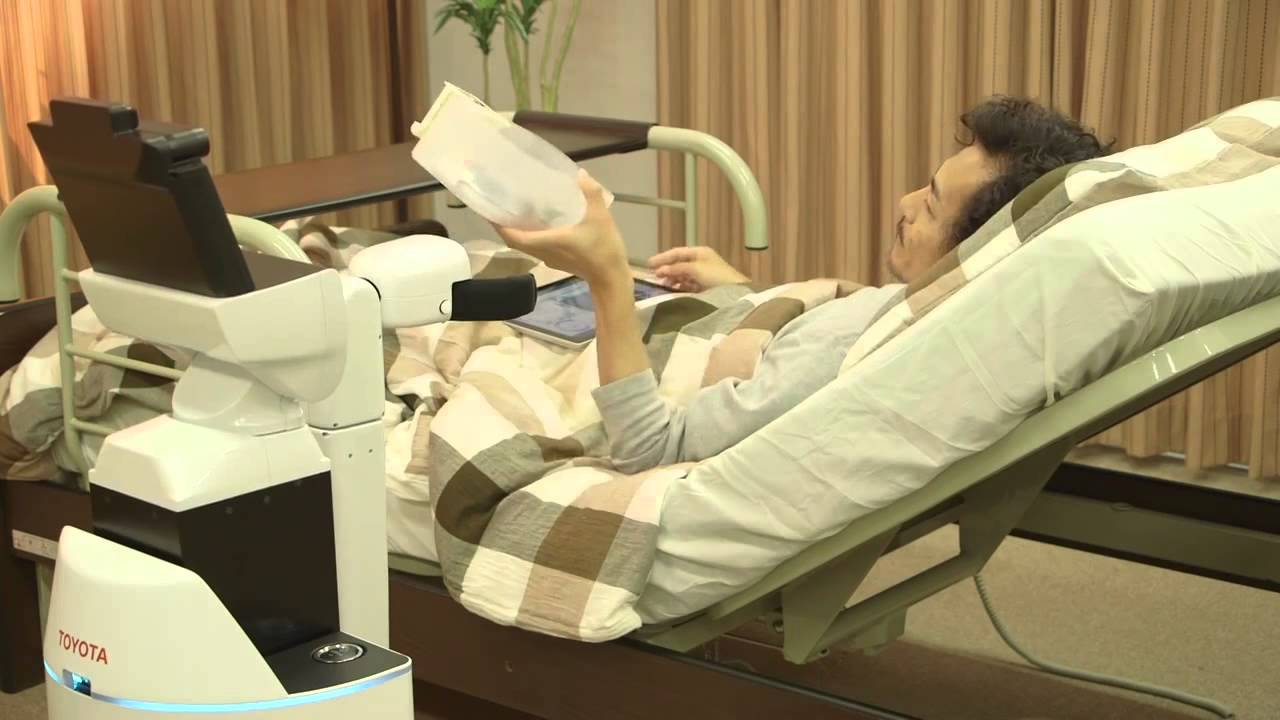
\includegraphics[width=5.0cm, height=3.5cm]{estadoArte/hsr_human_assistant_2.jpg}
		\end{subfigure}

		\caption{Robot de asistencia doméstica, desarrollado por la compañia Toyota (c). Asistente de tareas domésticas para personas con limitaciones físicas\cite{hsrEpage}.}
	\end{figure}

	En este contexto, se propone el desarrollo de herramientas tecnológicas que ayuden a mejorar la calidad de vida de la población que sufre alguna discapacidad en México. De acuerdo con la definición de robot de servicio propuesta por la FIR (Federación Internacional de Robótica), un robot de servicio diseñado, construido y programado para asistir en tareas domésticas podría ayudar a tal propósito. El hecho de tener un asistente doméstico podría significar delegar múltiples tareas a los robots. Estas tareas están orientadas a asistir a personas con problemas de motricidad, problemas de desplazamiento, problemas de memoria, entre otros. Un asistente doméstico ayudaría a la ejecución de estas actividades.\\ 

	Los robots enfrentan problemáticas a las que cualquier humano está sometido día a día: ambientes dinámicos, características de entornos no estandarizados, incertidumbre ante escenarios desconocidos. Dada la naturaleza de esta disciplina científica han surgido diversas líneas de investigación que abarcan estas problemáticas. La mecánica, la electrónica, la informática, la inteligencia artificial y la ingeniería de control, son algunas de las disciplinas involucradas. La robótica se ayuda de estas disciplinas para resolver problemas particulares, por ejemplo, un robot de servicios debe ser capaz de reconocer y manipular objetos en diferentes ubicaciones y desde diferentes alturas, tener locomoción en diferentes tipos de superficies, interactuar con un humano, distinguir diferentes personas, etc. Por último, pero no menos importante, el funcionamiento seguro de estos sistemas en ambientes dinámicos es un requisito fundamental para su futura aceptación y aplicabilidad.\\


	%¿Cual es la problematica?
	\section{Planteamiento del problema}

		%Problemática robots de servicio.
		La creación de estos sistemas autónomos requiere la integración de un gran conjunto de capacidades y tecnologías. Los ejemplos de capacidades incluyen la interacción humano-robot (habla, identificación de personas, seguimiento de personas, entre otros), navegación, planeación de acciones, control de comportamientos, detección, reconocimiento, manipulación o seguimiento de objetos. Con respecto a las tecnologías es requerida la aplicación de sensores RGB-D, cámaras estereoscópicas, sensores láser, entre otros.\\ 

		Con respecto a la inteligencia, los sistemas deben contener métodos de planificación de acciones y comportamientos adaptables. Los procedimientos apropiados deben, por ejemplo, permitir al operador enseñar al robot nuevos comportamientos y entornos vía comandos de voz o gestos. Los futuros hogares probablemente contendrán dispositivos electrónicos más inteligentes capaces de comunicarse entre si incluyendo el uso de internet como base común de conocimientos, de modo que los robots desempeñarán un papel más importante.\\
		%\vspace{0.2in}

		%Problemática de la manipulación
		Entre todas estas líneas de investigación es imprescindible contar con un robot que sea capaz de interactuar con los objetos en el mundo real, por ello es necesario contar un sistema que pueda reconocer los objetos y su posición adecuadamente. En el mundo real  los robots se enfrentan con condiciones dinámicas en el ambiente, por ejemplo al pedir a un robot que tome un objeto y pueda llevarlo hasta nosotros, el primer problema al que nos enfrentamos es conocer la posición del objeto (la cual será diferente en cada ocasión), posteriormente, si deseamos localizar dos objetos del mismo tipo, estos no serán reconocidos de igual manera por el robot debido a las condiciones de luz, a los cambios de forma, y a los cambios de apariencia.\\
		%\vspace{0.2in}

		En lo que respecta al proceso de la toma de objetos actual, en el robot de servicio Justina, unicamente se utiliza la información de posición del objeto sin considerar la información de orientación. Este proceso es susceptible a fallas cuando se trata de objetos de grandes dimensiones, entiendase objetos cuyas dimensiones son mayores a la longitud total del efector final del manipulador en su mayor apertura.\\


		%¿Cómo se solucionaria el problema?
		Dadas las condiciones antes descritas, es preciso contar con algoritmos que ayuden a mejorara la manipulación de objetos. Para ello es necesario dividir la tarea en operaciones: la primera de ellas consiste en estimar la posición del objeto, tener un indicador que nos ayude a determinar cuál es la mejor forma de tomar un objeto y contar con un algoritmo lo suficientemente robusto que lleve el efector final al objeto deseado. Otra de las operaciones necesarias es llevar el actuador final del brazo robótico a una posición (x, y, z) deseada. Por último es necesario contar con un planeador de acciones para coordinar cada uno de los eventos dentro de la tarea.\\
		%\vspace{0.2in}


		Podemos observar que las problemáticas son variadas, sin embargo podemos reducir el problema principal en tres tareas secundarias: Detectar un objeto, obtener una aproximación de cuál será la mejor manera de tomarlo y corroborar que el sistema de manipulación es robusto y óptimo en su ejecución.\\
		%\vspace{0.2in}


	\section{Hipótesis}
		\begin{itemize}

			\item Un sistema de visión computacional con implementación de un algoritmo de análisis de componentes principales podrá indicarnos cuál es la mejor orientación para tomar un objeto y por tanto mejorará la manipulación de objetos.\\
			%\vspace{0.25in}

		\end{itemize}

	\section{Objetivos}
		\subsection*{Objetivo general}
			Implementar un conjunto de algoritmos de visión computacional que mejore el sistema de detección y manipulación de objetos formado por un sensor kinect y un brazo robótico de 7DOF en un robot de servicios.
		\subsection*{Objetivos específicos}
			\begin{itemize}
				\item Implementar un algoritmo de visión computacional para identificar un plano.

				\item Implementar un algoritmo de visión computacional para determinar la posición de un objeto.

				\item Implementar un algoritmo de análisis de componentes principales para calcular la orientación de un objeto.

				\item Caracterizar el espacio de trabajo del manipulador de 7DOF ubicado en el robot de servicio Justina.

				\item Poner a prueba dos diferentes algoritmos para el cálculo de la cinemática inversa de un brazo robótico de 7DOF, un algoritmo geométrico y un algoritmo numérico.

				\item Realizar pruebas de desempeño para verificar si existe una mejora significativa entre las tareas.

			\end{itemize}

	% \newpage{}

	\section{Descripción del documento}
	%¿Qué encontraremos en el documento?
	En el capítulo 2 de este documentos se definen los conceptos utilizados para la solución propuesta. En el capítulo 3 se aborda la manera en que se desarrollaron los algoritmos de visión computacional para realizar la extracción de un plano, identificar la posición de un objeto, implementar un algoritmo de Análisis de Componentes Principales (PCA por sus siglas en inglés) para obtener cual será la mejor orientación para tomar un objeto a partir de su forma. En el capítulo 4 se describe el sistema de manipulación utilizado en este trabajo de tesis. Se comienza por conocer las características de los actuadores utilizados, se obtienen las ecuaciones correspondientes a la cinemática de los brazos para llevarlo hasta una posición (x, y, z, roll, pitch, yaw) deseada. En el capítulo 5 se realiza la descripción de las tareas antes mencionadas, la plataforma sobre la cual se desarrolló el sistema y la implementación del sistema de manipulación de objetos en un robot de servicios. En el capítulo 6 se reportan los resultados y conclusiones obtenidos de este trabajo.\\

\newpage
\thispagestyle{empty}
\mbox{}
\addtocounter{page}{-2}
